%(BEGIN_QUESTION)
% Copyright 2015, Tony R. Kuphaldt, released under the Creative Commons Attribution License (v 1.0)
% This means you may do almost anything with this work of mine, so long as you give me proper credit

Ha det litt gøy med å skrive enkle «utforskings-» eller «demonstrasjons-»programmer i ladderdiagram for PLC, for å utføre ulike funksjoner. Prøv gjerne følgende instruksjonstyper:

\begin{itemize}
\item{} Kontakter og spoler
\item{} Tellere (opp, ned, opp/ned)
\item{} Timere (innkoblingsforsinkelse, utkoblingsforsinkelse, retentiv)
\item{} Sekvenseringsinstruksjoner
\item{} Matematiske instruksjoner (addisjon, subtraksjon, multiplikasjon, divisjon)
\end{itemize}

Identifiser realistiske anvendelser for PLC-programmer med tellere og timere. Hvilke prosesser i virkeligheten kan ha nytte av en PLC-funksjon der noe slår seg av eller på etter et bestemt antall pulser på en inngang, eller etter at en viss tid har gått?

\vskip 10pt

{\bf Merk: Denne enkle øvelsen kan virke triviell, men den er nøkkelen til selvstendig læring i PLC-programmering.} Å ha en egen PLC å jobbe med i klasserommet er et svært kraftig læringsverktøy. Når du møter en ny instruksjon (for eksempel timer eller matematikk-instruksjon) som du ennå ikke kan bruke, kan du utforske egenskaper og oppførsel ved å lage et enkelt program i PLC-en med bare denne instruksjonen. PLC-ens {\it User Manual} eller {\it Instruction Set}-manual viser grunnsyntaksen, som du kan bruke som eksempel. Når programmet er lastet inn i PLC-minnet, kan du «leke» med det og observere oppførselen online.

Når du har observert hvordan instruksjonen virker, er neste steg å legge inn kommentarer i programmet som beskriver virkemåten med dine egne ord. Vær detaljert, og skriv som om du skulle forklart alt til en person som ikke kan noe om instruksjonen. Disse kommentarene blir notater til deg selv, når du senere må friske opp minnet om hvordan en bestemt instruksjon fungerer og hva den brukes til.

\vskip 10pt

{\it Ikke bli overrasket hvis instruktøren senere ber deg vise demonstrasjonsprogrammene dine for bestemte instruksjoner. Hvis du har vansker med en instruksjon i en programmeringsoppgave, kan instruktøren sjekke om du har laget og kjørt et demonstrasjonsprogram for å lære hvordan instruksjonen faktisk skal virke.}

\vskip 10pt

Se «Answer»-delen i denne oppgaven for eksempler på hvordan et slikt demonstrasjonsprogram kan se ut.

\vskip 20pt \vbox{\hrule \hbox{\strut \vrule{} {\bf Forslag til sokratisk diskusjon} \vrule} \hrule}

\begin{itemize}
\item{} Et nyttig tips når du lager egne demonstrasjonsprogrammer er å lagre hvert program med filnavn som er lette å finne igjen på PC-en. Du kan for eksempel starte alle slike filer med ordet «Demo» og bruke understrek mellom beskrivende ord (eller instruksjonsnavn). Noen eksempler:
\begin{itemize}

\item{} {\tt Demo\_upcounter}
\item{} {\tt Demo\_downcounter}
\item{} {\tt Demo\_TOF\_timer}
\item{} {\tt Demo\_TON\_timer}
\item{} {\tt Demo\_ADD\_instruction}
\end{itemize}
\end{itemize}

\underbar{file i00120}
%(END_QUESTION)





%(BEGIN_ANSWER)

\noindent
{\bf Demonstrasjonsprogram som viser noen grunnleggende bit-instruksjoner i en Allen-Bradley MicroLogix PLC:}

$$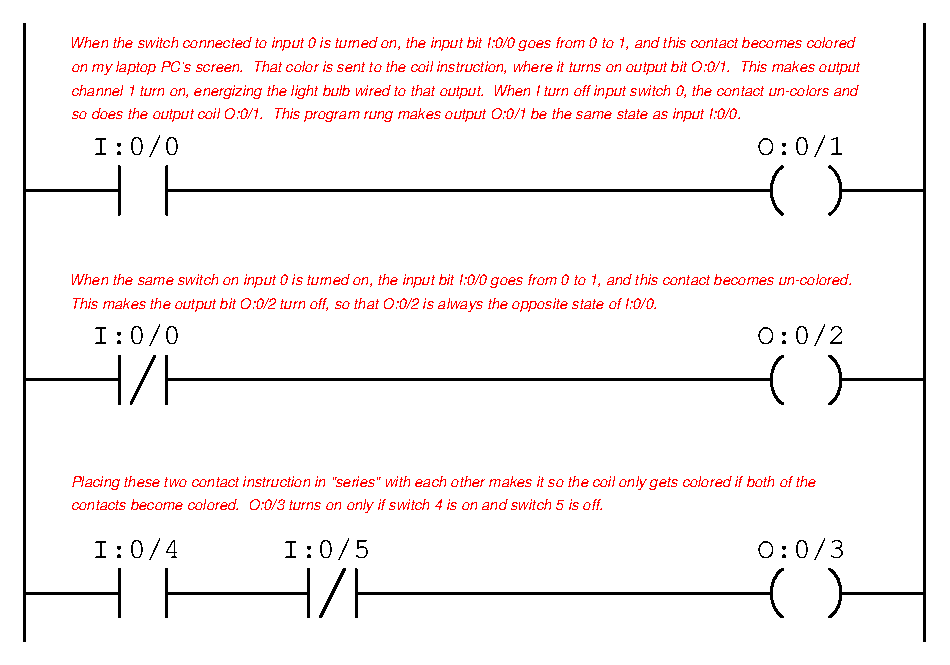
\includegraphics[width=15.5cm]{i00120x01.eps}$$


\filbreak

\noindent
{\bf Demonstrasjonsprogram som viser «opp»- og «ned»-tellerinstruksjoner i en Allen-Bradley MicroLogix PLC:}

$$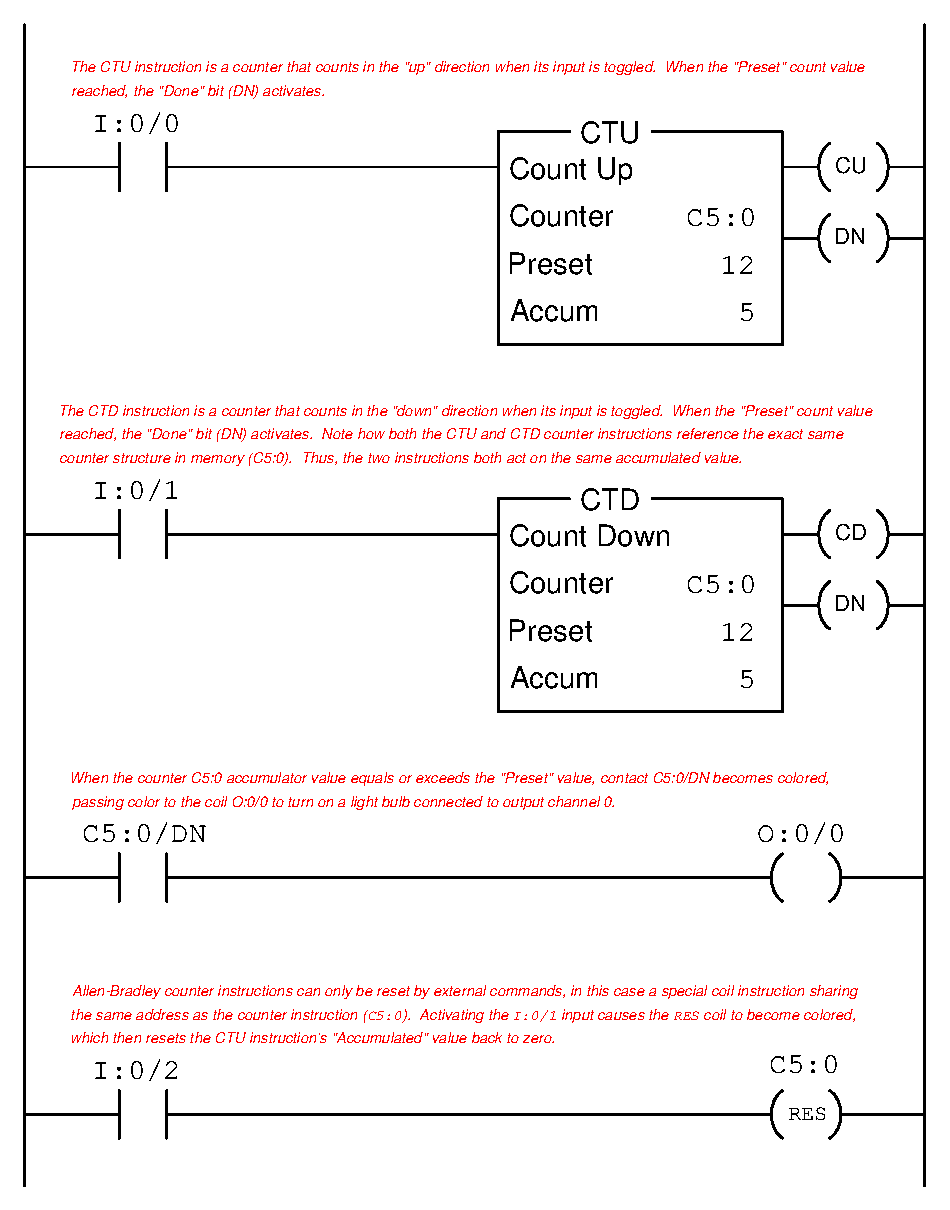
\includegraphics[width=15.5cm]{i00120x03.eps}$$


\filbreak

\noindent
{\bf Demonstrasjonsprogram som viser en innkoblingsforsinket timerinstruksjon i en Allen-Bradley MicroLogix PLC:}

$$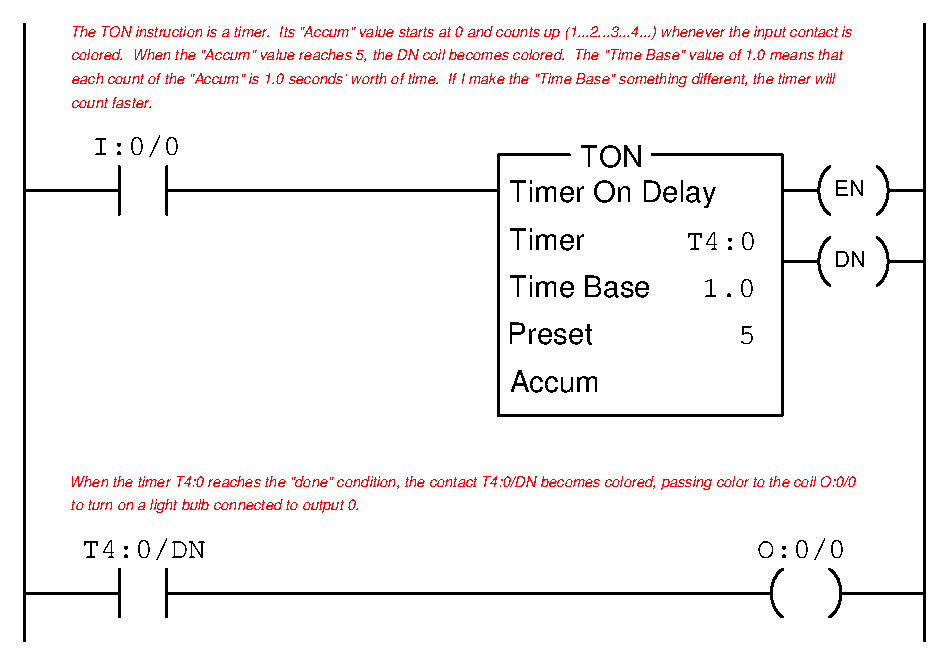
\includegraphics[width=15.5cm]{i00120x02.eps}$$

%(END_ANSWER)





%(BEGIN_NOTES)

\vfil \eject

\noindent
{\bf Oppsummeringsquiz:}

Denne øvelsen egner seg svært godt som oppsummeringsquiz: la studenten vise minst ett nytt demonstrasjonsprogram, fullt kommentert og i drift. Oppmuntre til utfyllende kommentarer, slik at rung-kommentarene blir så tydelige at hvem som helst kan lære instruksjonen ved å lese dem. {\it Be studenten bokstavelig demonstrere hva som er lært ved å kjøre programmet og forklare hva instruksjonen gjør online (med statusfarger og tallverdier vist direkte).}

\vskip 10pt

{\it Minn studentene om at du (som instruktør) vil få dem til å bruke demonstrasjonsprogrammene hvis de senere får problemer med en bestemt instruksjon. Hensikten er å bygge en god vane med demonstrasjonsprogrammer for selvstyrt PLC-læring, og samtidig sikre at programmene er dokumentert godt nok til å være nyttige ved framtidige spørsmål og problemer.}

\vskip 10pt

I min erfaring som lærer motsetter mange studenter seg å lage demonstrasjonsprogrammer, fordi de tror slike øvelser er bortkastet tid og at de lærer bedre ved å få en direkte forklaring av instruktøren. Det som ofte skjer når instruktøren bare forklarer, er imidlertid at de samme studentene kommer tilbake med det samme spørsmålet senere (fordi de egentlig ikke lærte det første gang). Når studenter lærer å skrive egne demonstrasjonsprogrammer, lærer de å lære seg PLC-programmering selv, og det er en mye mer verdifull og varig ferdighet enn målrettet enkelthjelp fra instruktøren.



%INDEX% PLC, exploratory question (ladder logic programming with counters and timers)

%(END_NOTES)
